\subsection{So sánh các giải pháp Networking}
Hiện nay, trên thị trường có nhiếu công cụ (framework) hỗ trợ lập trình multiplayer cho Unity rất mạnh mẽ. Trong đó có những công cụ bên thứ ba có thể tích hợp vào Unity như \textbf{Photon} (PUN, Fusion, Quantum), \textbf{Mirror Networking} và cũng có những công cụ do chính Unity phát triển như \textbf{Netcode for GameObjects} (NGO), \textbf{Netcode for Entities}. Sau đây, nhóm sẽ phân tích và so sánh các giải pháp trên nhằm đưa ra được lựa chọn hợp lý cho công cụ lập trình Networking của dự án.
\subsubsection{Photon}
    Trong Photon có 3 giải pháp chính cho Networking là PUN (Photon Unity Networking), Fusion và Quantum. Dưới đây là so sánh tổng quan về 3 giải pháp trên.

    \begin{table}[H]
        \centering
        \begin{tabular}{|c|M{3cm}|M{3.5cm}|M{3cm}|} 
            \hline
                \textbf{Đặc điểm} & \textbf{PUN} & \textbf{Fusion} & \textbf{Quantum} \\
                \hline
                Cơ chế đồng bộ & State sync (thủ công cổ điển) & Snapshot-based (Host mode/Dedicated Server) & Deterministic lockstep\\
                \hline
                Độ khó sử dụng & Dễ & Trung bình & Khó \\
                \hline
                Độ trê & Trung bình & Thấp & Cực thấp \\
                \hline
                Ưu điểm & Dễ dùng, nhiều tài liệu hướng dẫn & Hiệu năng tốt hơn PUN, hỗ trợ rollback, prediction & Hiệu năng cao nhất, chống gian lận, đa nền tảng \\
                \hline
                Nhược điểm & Chậm, đã ngừng phát triển & Cần nhiều kiến thức networking hơn & Phải code ESC theo kiểu của Quantum\\
                \hline
                Dòng game phù hợp & Casual, board game (nhẹ, ít vật thể) & FPS, 3D action (yêu cầu realtime, nhiều tác động vật lý) & MOBA, Fighting (cần đột chính xác rất cao, anti-cheat)\\
                \hline
        \end{tabular}
        \caption{So sánh 3 giải pháp Photon hỗ trợ}
        \label{tab:photon}
    \end{table}

    
    \begin{figure}[!h]
    \centering
    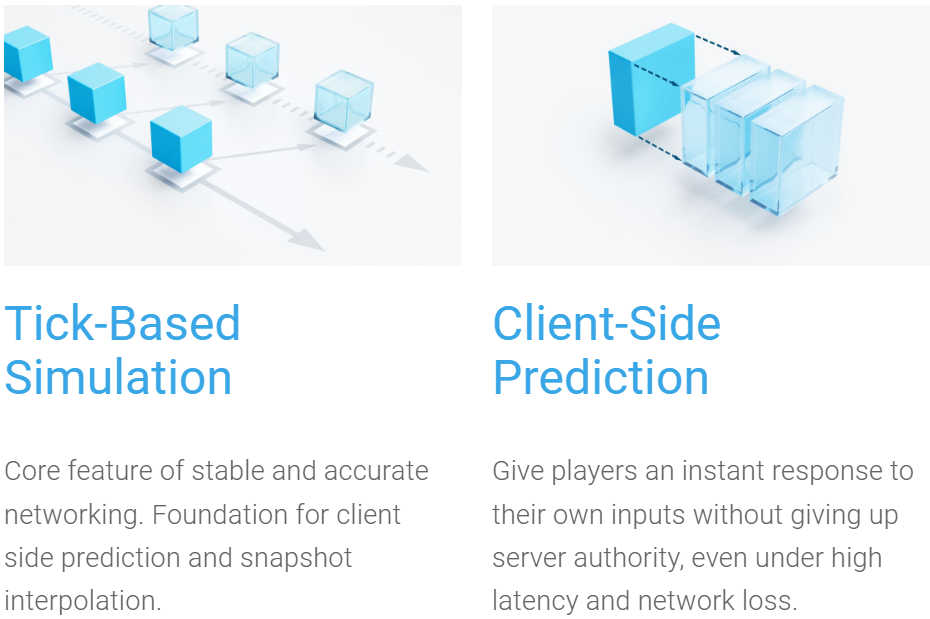
\includegraphics[width=8cm]{4.Cơ sở/images/fusion-1.png}
    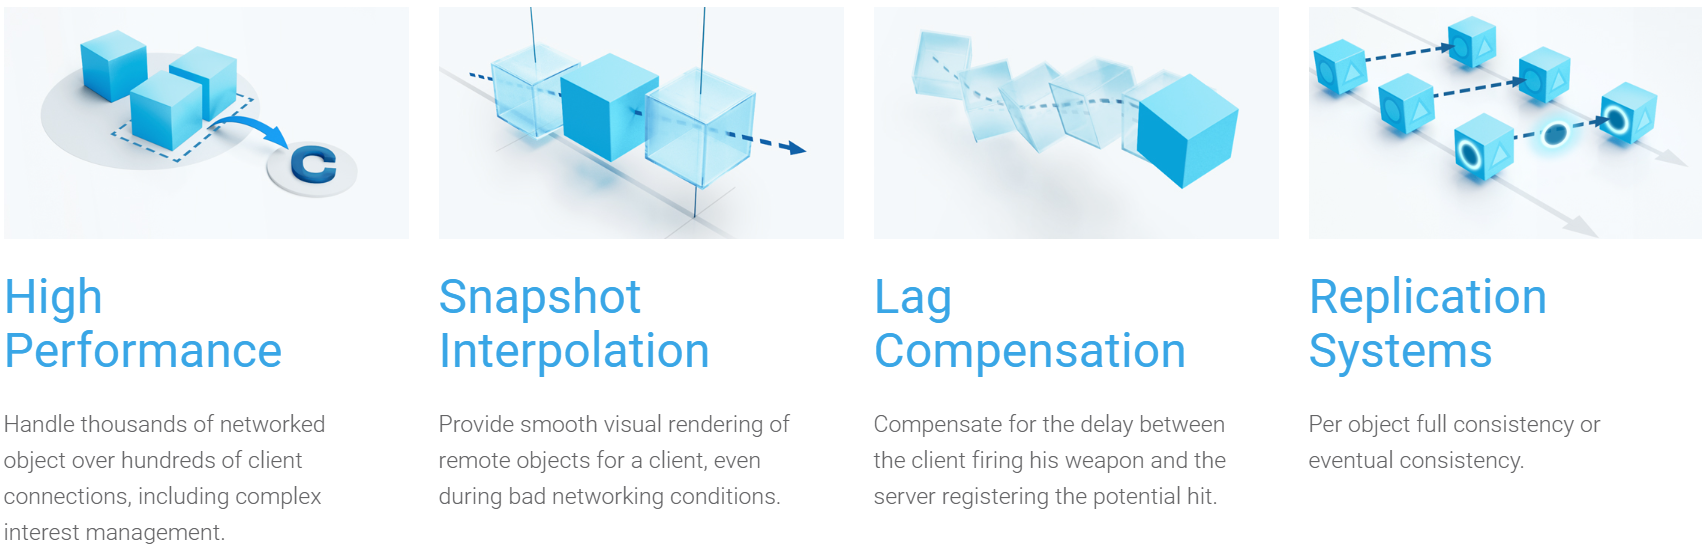
\includegraphics[width=12cm]{4.Cơ sở/images/fusion-2.png}
    \caption{Tính năng chính của Photon Fusion}
    \label{fig:fusion}
    \end{figure}

% Nếu gói subcaption gây lỗi, hãy thử dùng gói subfigure: \usepackage{subfigure}

\begin{figure}[!h]
    \centering
    \begin{minipage}{0.35\textwidth} 
        \centering
        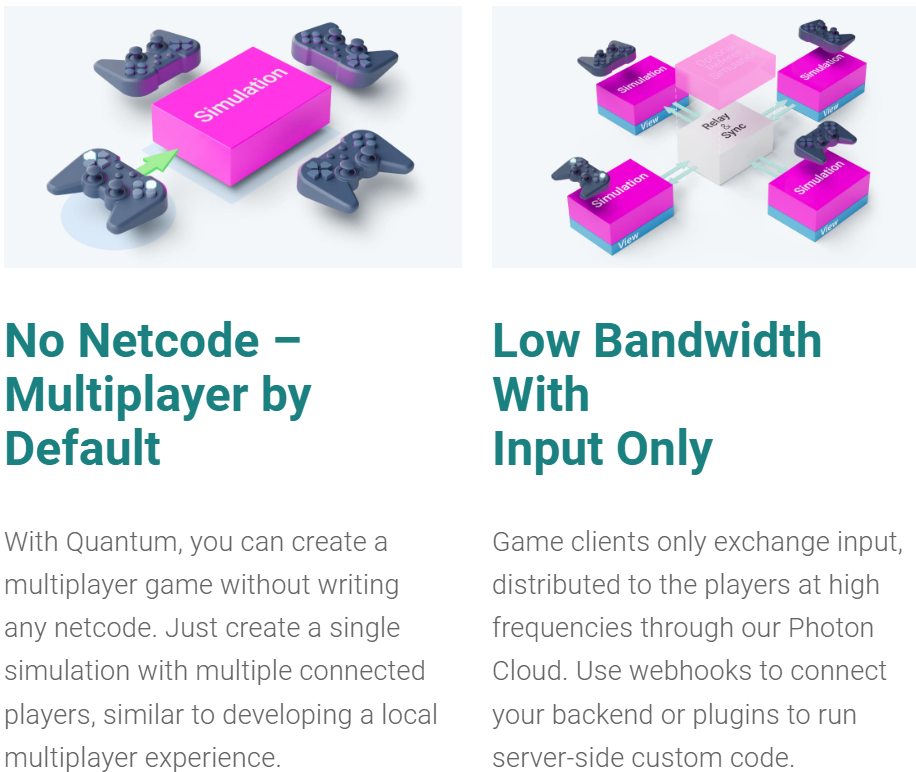
\includegraphics[width=\linewidth]{4.Cơ sở/images/quantum-1.png}
    \end{minipage}
    \begin{minipage}{0.35\textwidth} 
        \centering
        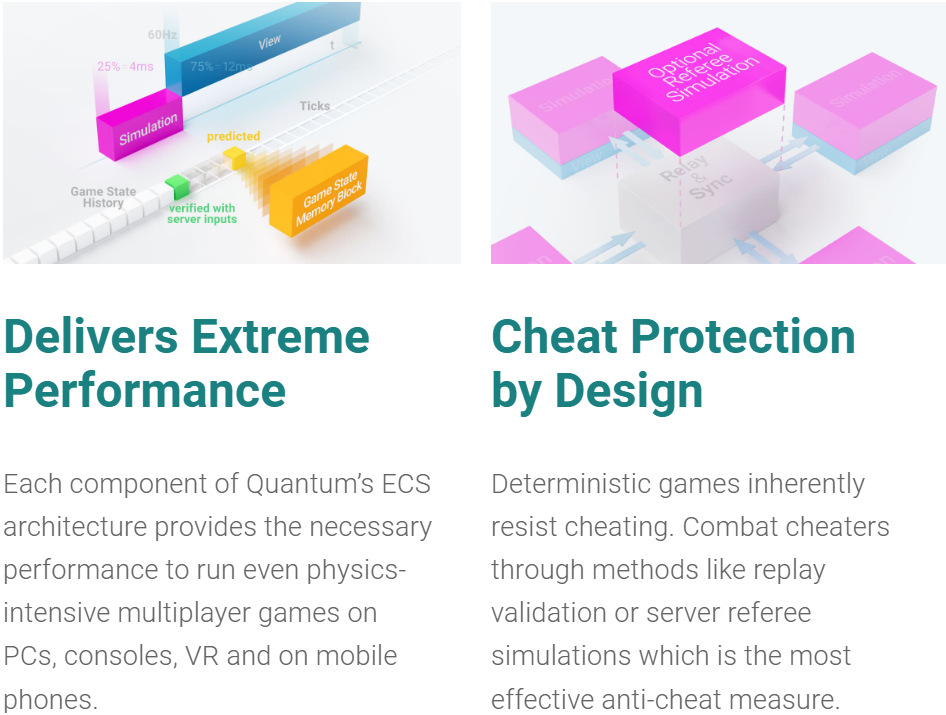
\includegraphics[width=\linewidth]{4.Cơ sở/images/quantum-2.png}
    \end{minipage}
    \centering
    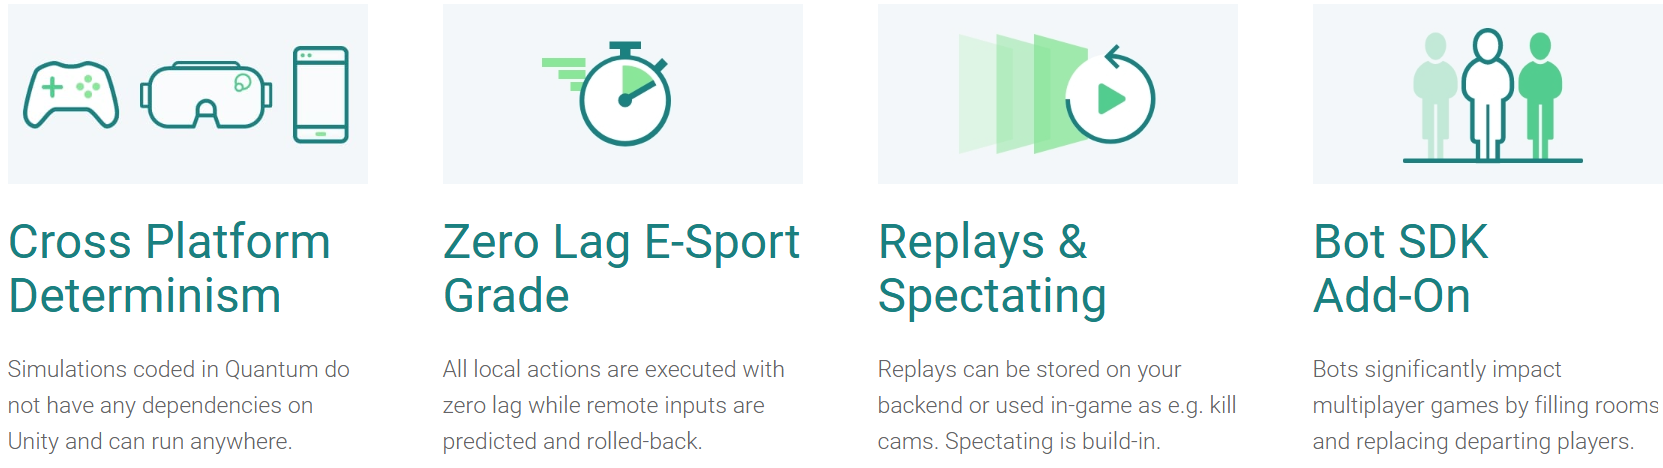
\includegraphics[width=12cm]{4.Cơ sở/images/quantum-3.png}

    \caption{Tính năng chính của Photon Quantum}
    \label{fig:fusion}
\end{figure}
    
    Hiện tại, các giải pháp trên của Photon đều cung cấp gói miễn phí với giới hạn số người dùng trực truyến cùng lúc (CCU) tối đa là 20 và chỉ dành cho phiên bản phát triển (development only). 

    \begin{figure}[!h]
    \centering
    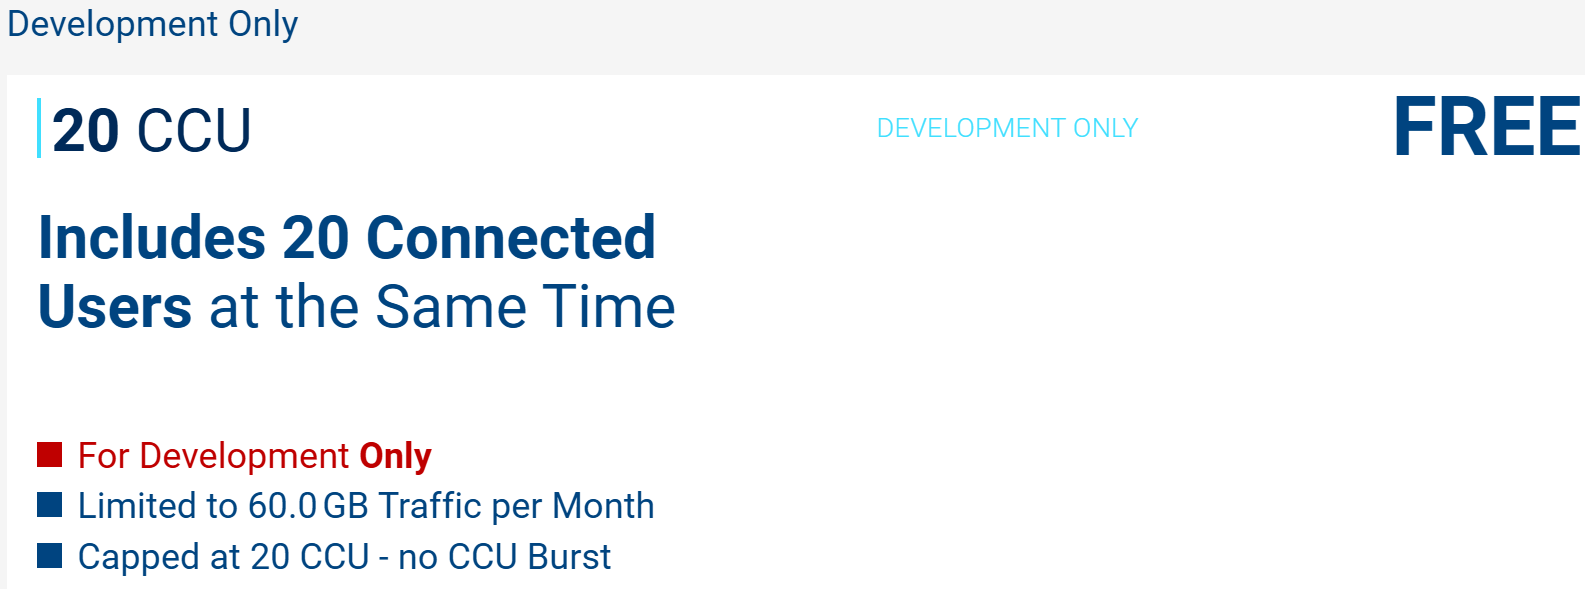
\includegraphics[width=12cm]{4.Cơ sở/images/photon-price-1.png}
    \caption{Gói dịch vụ miễn phí của Photon (PUN, Fusion, Quantum) cho bản phát triển}
    \label{fig:photon-price-1}
    \end{figure}
    
    Riêng công cụ Fusion và Quantum thì có thêm 1 gói miễn phí cho phiên bản phát hành (chỉ 1 app duy nhất) với giới hạn CCU tối đa lên đến 100 kèm theo tăng traffic mỗi tháng (từ 60GB lên 0.3TB).
    \begin{figure}[!h]
    \centering
    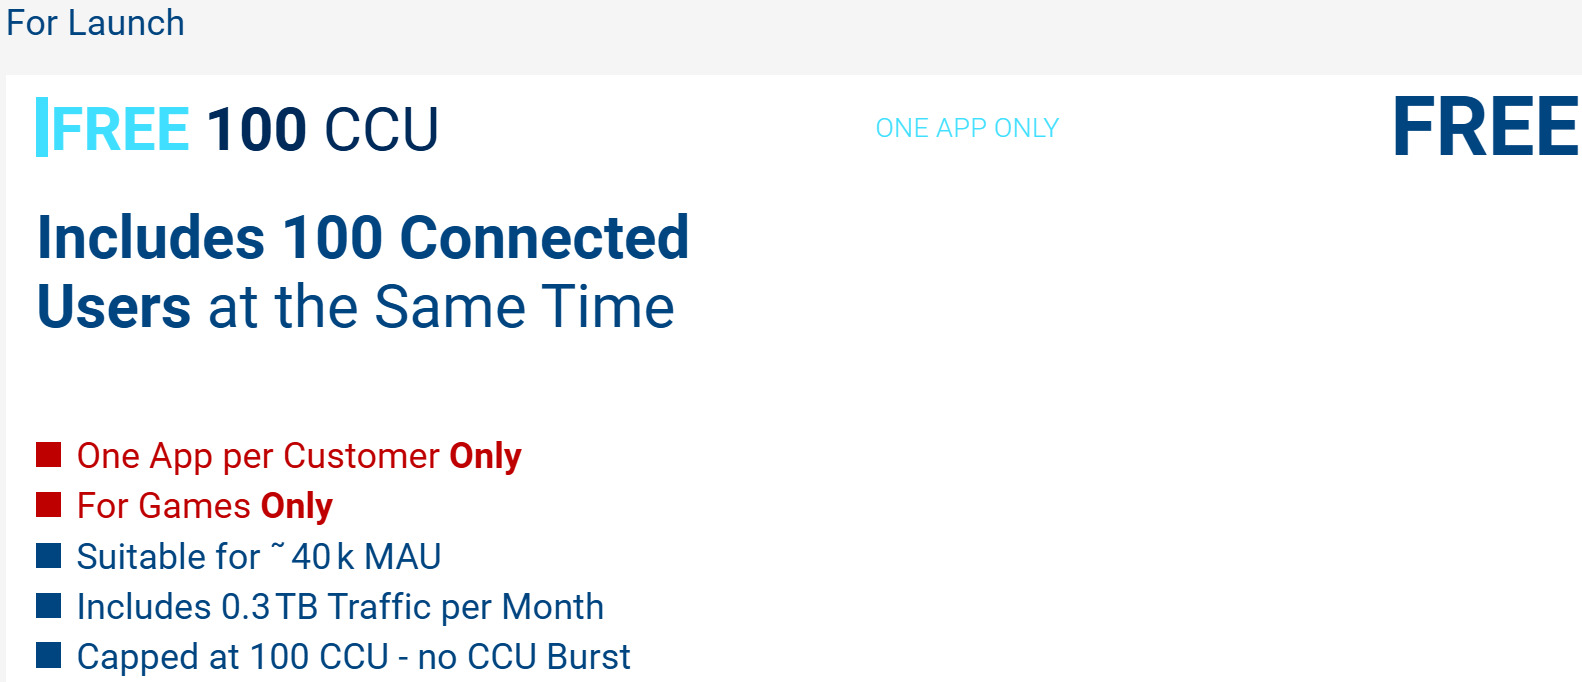
\includegraphics[width=12cm]{4.Cơ sở/images/photon-price-2.png}
    \caption{Gói dịch vụ miễn phí của Photon (Fusion, Quantum) cho bản phát hành}
    \label{fig:photon-price-2}
    \end{figure}
    
    Các gói dịch vụ cao cấp hơn của Photon (mở giới hạn traffic, CCU) phải trả phí (95\$/12 tháng, 125\$/tháng, 250\$/tháng, 500\$/tháng) 
    \begin{figure}[!h]
    \centering
    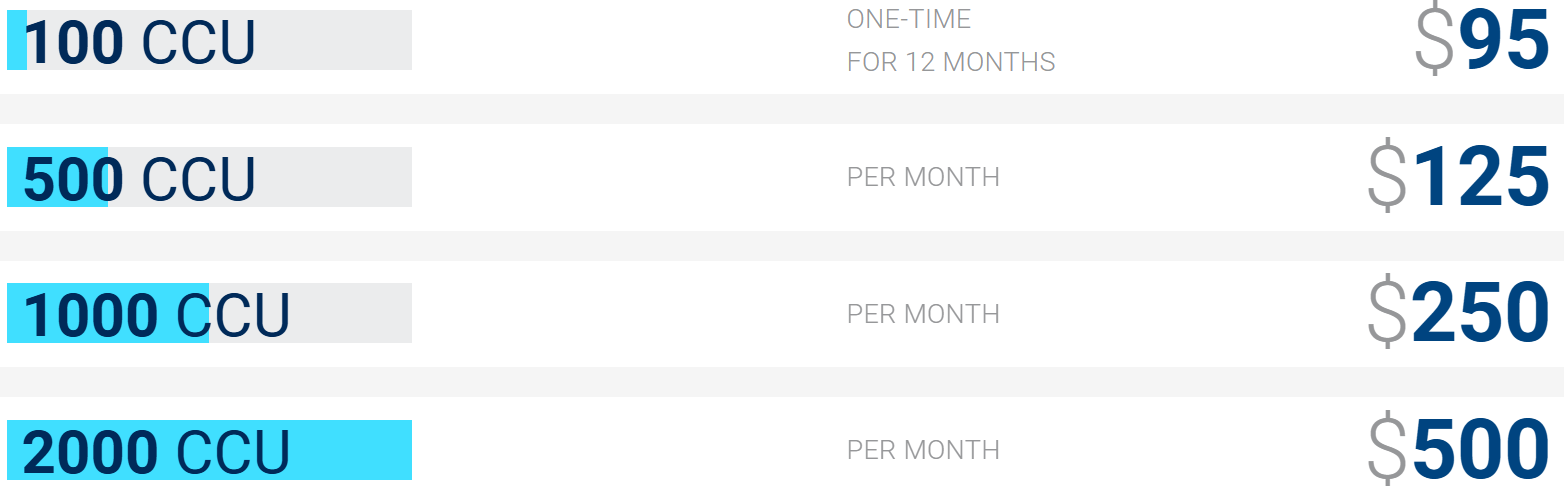
\includegraphics[width=12cm]{4.Cơ sở/images/photon-price-3.png}
    \caption{Gói dịch vụ trả phí của Photon (PUN, Fusion, Quantum)}
    \label{fig:photon-price-3}
    \end{figure}
    
\newpage
\subsubsection{Mirror Networking:}
Mirror Networking là một thư viện mã nguồn mở dùng cho networking trong Unity. Thư viện này hoàn toàn miễn phí và luôn được cập nhật đều đặn đến hiện tại. Mirror Networking hô trợ host mode (P2P) và cả dedicated server. Nhờ những đặc tính của một thư viện mã nguồn mở, công cụ này cung cấp khả năng linh hoạt, tùy biến cao. Điều này phù hợp cho nhóm phát triển nhỏ (indie), yêu cầu cao cho việc kiểm soát logic server, mạng chặt chẽ, mở rộng tùy ý. Giải pháp này không giới hạn về CCU, nhưng sẽ phụ thuộc vào cấu hình server mà nhà phát triển xây dựng.
\subsubsection{Netcode for GameObjects (NGO)}
NGO (Netcode for GameObjects) là một công cụ chính thức được Unity phát triển và là giải pháp mặc định cho quá trình phát triển game Multiplayer trong unity. NGO có giao diện sử dụng dễ dàng, thân thuộc nhờ việc xây dựng trên workflow truyền thống của Unity (GameObject, MonoBehaviour,...). 

Các dịch vụ Multiplayer khác của Unity cũng được tích hợp vào NGO:
\begin{itemize}
    \item Lobby: có thể hỗ trợ lên đến 150 người chơi 1 phòng
    \item Player Authentication: xác thực người dùng đa nền tảng (facebook, google, anonymous,...)
    \item Matchmaker: hỗ trợ cơ chế ghép trận
    \item Relay: hỗ trợ cho P2P
    \item Friends; hỗ trợ cơ chế bạn bè
    \item Vivox: hỗ trợ cơ chế voice chat, text chat
\end{itemize}

NGO hỗ trợ 2 kiến trúc mạng chính là Client-Server (Dedicated server) và Client-Host. Về giao thức truyền tải mạng, NGO sử dụng UPD đạng tin cậy (Reliable UDP), giao thức này vừa kế thừa đặc điểm tốc độ cao của UDP truyền thống, vừa kết hợp đặc tính tin cậy (tính đảm bảo chuyển giao, tính thứ tự) của giao thức TCP.\\

Với gói dịch vụ miễn phí, NGO cung cấp giới hạn CCU tối đa mỗi tháng lên đến 50 và với mỗi mốc vượt ngưỡng sẽ trả phí (pay as you go).
\begin{figure}[!h]
    \centering
    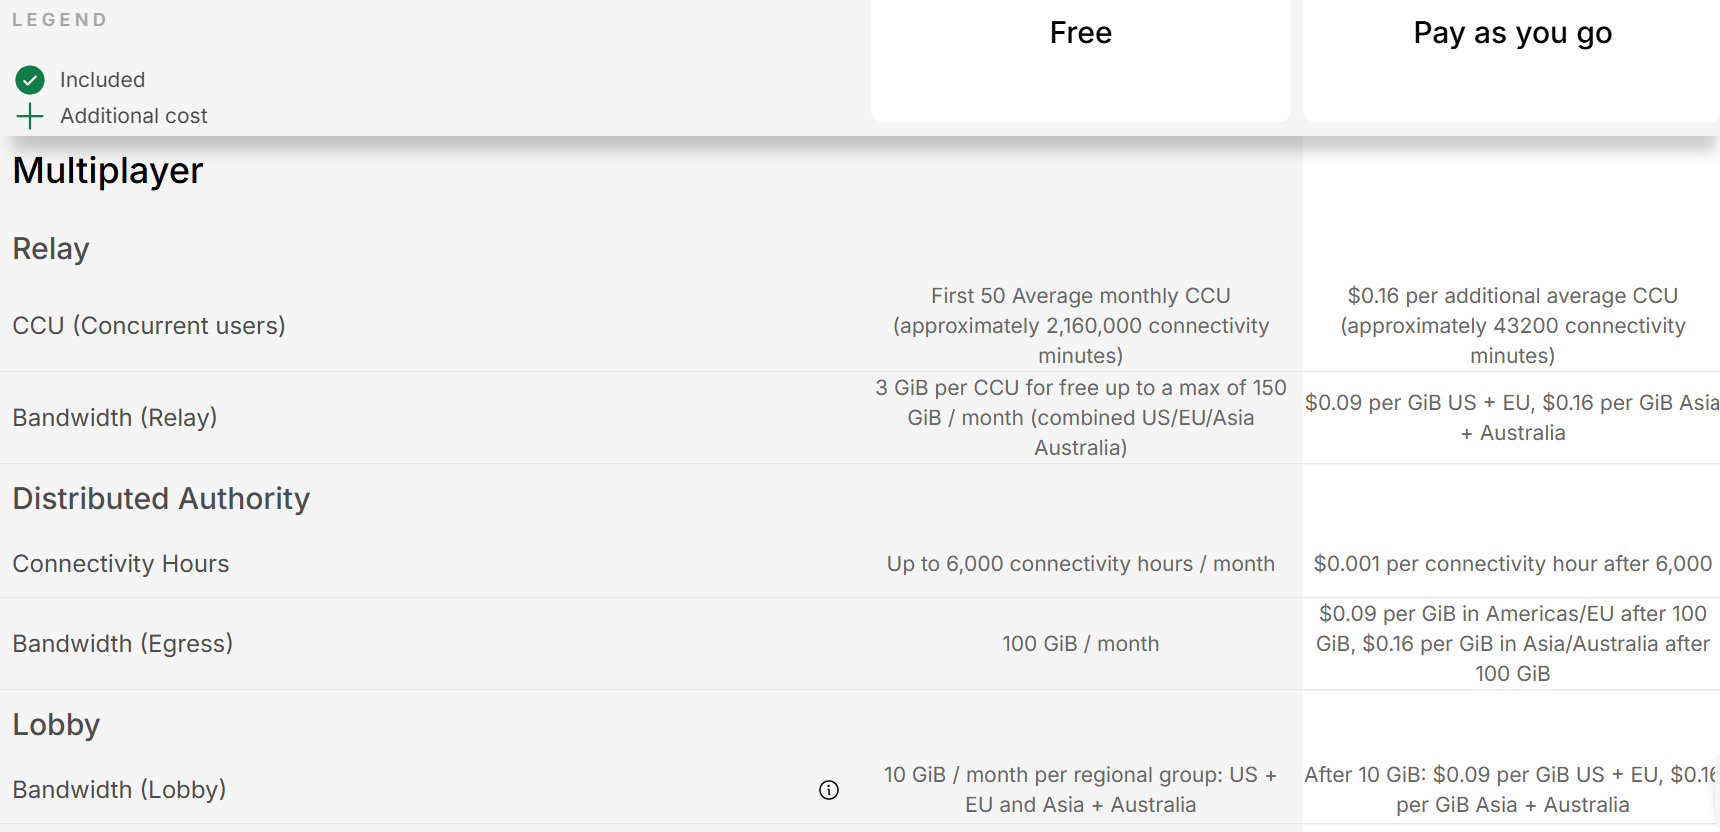
\includegraphics[width=12cm]{4.Cơ sở/images/ngo-price.png}
    \caption{Gói dịch vụ cho Multiplayer của Unity}
    \label{fig:ngo-price}
\end{figure}

Tuy hỗ trợ nhiều dịch vụ, nhưng hệ thống của NGO chỉ phù hợp cho dự án quy mô nhỏ (khoảng 8-16 người chơi 1 phòng). Với các game có số lượng người chơi lớn, hiệu suất của NGO sẽ giảm mạnh. Ngoài ra, NGO cũng không hỗ trợ Client-side Prediction và Lag Compensation, điều này gây khó khăn trong việc hiện thực các game hành động nhanh, FPS khi nhà phát triển phải tự triển khai toàn bộ, làm tăng độ phức tạp của dự án.
\subsubsection{Netcode for Entities}
Tương tự NGO, Netcode for Entities cũng là một công cụ chính thức do Unity phát triển. Tuy nhiên, công cụ này tập trung tối ưu cho những game đòi hỏi số lượng người chơi lớn, xử lý nhiều logic, vật lý cho nhiều vật thể cùng lúc. Netcode for Entities được dùng kết hợp với hệ thống ECS (Entity Component System) và DOTS (Data-Oriented Technology Stack) để tối ưu hiệu suất xử lý đồng thời nhiều đối tượng. Ngoài ra, công cụ này cũng có thể dễ dàng tích hợp với dịch vụ của Unity như NGO.